\documentclass{article}

% ---------- NeurIPS-style formatting ----------
\usepackage[final]{neurips_2024}

\usepackage[utf8]{inputenc}
\usepackage[T1]{fontenc}
\usepackage{amsmath,amssymb,amsfonts}
\usepackage{mathtools}
\usepackage{booktabs}
\usepackage{graphicx}
\usepackage{hyperref}
\usepackage{cleveref}
\usepackage{subcaption}
\usepackage{xcolor}
\usepackage{multirow}

% ---------- Notation ----------
\newcommand{\R}{\mathbb{R}}
\newcommand{\poinc}{\mathbb{B}^{d}_{c}}
\newcommand{\dH}{d_{\poinc}}
\DeclareMathOperator{\KL}{KL}

\title{What Does the Model Learn About the Curvature?\\
An Empirical Study of Learned Poincar\'{e} Curvature\\
in Hyperbolic Zero-Shot Learning}

\author{
  Ilir Bejleri \\
  \texttt{ibejler3@gatech.edu}
}

\begin{document}

\maketitle

% ================================================================
%  ABSTRACT
% ================================================================
\begin{abstract}
A prior result on AwA2~\cite{bejleri2025bayesian} reported that the learnable curvature $c$ of a Poincar\'{e} ball hyperbolic zero-shot learning model scaled monotonically with training data, suggesting a universal $c \propto \log N$ relationship.
We test this on seven image classification datasets spanning attribute-based and text-based class embeddings, and from very flat (Stanford Cars) to deeply hierarchical (iNaturalist, tiered-ImageNet) label spaces.
We find that the relationship is \emph{not} universal.
Across the seven datasets, the per-dataset slope of $c$ vs.\ $\log N$ varies from $+1.31$ ($R^2=0.95$, AwA2) all the way to $-0.17$ ($R^2=0.86$, SUN397) --- a directionally inconsistent range that decisively rules out a single scaling law.
Instead, we identify three distinct response patterns:
(1) \emph{strongly increasing} curvature with data (AwA2);
(2) \emph{rising then plateauing} curvature (CUB-200, Stanford Cars, CIFAR-100);
(3) \emph{peaking early then declining} curvature (SUN397, iNaturalist, tiered-ImageNet).
The single biggest determinant of which pattern a dataset exhibits is the \emph{type} of class embedding used, not its taxonomy depth: AwA2 uses 85-d expert-annotated binary attributes (e.g., \texttt{has\_stripes}, \texttt{carnivorous}), while every other dataset uses 300-d GloVe word vectors derived from class names.
We argue that learned curvature reports the dataset's \emph{available semantic structure} as seen through the chosen embedding, not its underlying taxonomy depth.
This finding has consequences for the recent generalisation results of Fan et al.~\cite{fan2025curvature}: their reported optimal curvature should be interpreted relative to the embedding modality, not as a property of the dataset's classes per se.
\end{abstract}

% ================================================================
%  1. INTRODUCTION
% ================================================================
\section{Introduction}\label{sec:intro}

Hyperbolic spaces are natural targets for embedding hierarchical data~\cite{nickel2017poincare,nickel2018learning}, and modern hyperbolic neural networks~\cite{ganea2018hyperbolic,becigneul2019riemannian,kochurov2020geoopt} commonly treat the Poincar\'{e} ball curvature $c$ as a learnable parameter rather than a fixed hyperparameter.
A natural question is what the model is doing when it learns this parameter --- in particular, what information about the dataset is encoded in the converged value.

In an earlier paper, we trained a Bayesian hyperbolic zero-shot learning (ZSL) model on AwA2 across a data-ablation sweep and observed that $c$ scaled monotonically with training set size, from $c = 1.18$ at 1\% data to $c = 6.63$ at 100\%~\cite{bejleri2025bayesian}.
The relationship looked clean enough on a $\log$ scale to invite a strong reading: that learnable curvature obeys a universal $c \propto \log N$ scaling law, with the slope and intercept perhaps controlled by hierarchy depth.
This paper tests that reading.

\paragraph{What we did.}
We trained the same model architecture --- with no hyperparameter changes --- on seven image classification datasets covering a wide range of taxonomic structures and class-embedding modalities: AwA2~\cite{xian2018awa2}, CIFAR-100~\cite{krizhevsky2009cifar}, CUB-200~\cite{wah2011cub}, SUN397~\cite{xiao2010sun}, Stanford Cars~\cite{krause2013cars}, iNaturalist~\cite{vanhorn2021inaturalist}, and tiered-ImageNet~\cite{ren2018tiered}.
Each was run through the same data-ablation sweep at $\{1, 5, 10, 25, 50, 100\}\%$ of the training set.

\paragraph{What we found.}
The $c \propto \log N$ pattern does \emph{not} generalise.
Fitting $c = a \log N + b$ separately per dataset, the slope $a$ varies from $+1.31$ (AwA2) to $-0.17$ (SUN397), changing sign across the seven datasets.
The within-dataset trajectories cluster into three qualitatively distinct response patterns (\Cref{sec:patterns}):
\begin{enumerate}
    \item \textbf{Monotonic increase} --- AwA2 is the only dataset in this group, climbing 5.6$\times$ from 1\% to 100\% data.
    \item \textbf{Rise then plateau} --- CUB-200, Stanford Cars, and (loosely) CIFAR-100. Curvature rises to a moderate ceiling around $c \in [1.6, 2.3]$ by 25\% data, then stays flat or drifts down slightly.
    \item \textbf{Peak then decline} --- SUN397, iNaturalist, and tiered-ImageNet. Curvature peaks early (often at 5--10\% data) and then \emph{decreases}, sometimes ending below its initial value.
\end{enumerate}
The taxonomy-depth ordering of the datasets does not predict which group a dataset falls into.
The strongest predictor we identify is the \emph{class-embedding modality}.
AwA2 is the only dataset using expert-annotated per-class binary attributes (85-d, e.g., \texttt{has\_stripes}, \texttt{carnivorous}); the other six use 300-d GloVe word vectors~\cite{pennington2014glove} derived from class names.
The 4$\times$ gap between AwA2's converged curvature ($c=6.63$) and the next-highest dataset (CIFAR-100, $c=1.81$) lines up with this distinction far more cleanly than with anything taxonomic.

\paragraph{What it means.}
We re-frame the original question.
Rather than asking ``what does converged curvature reveal about the dataset?'', the right question appears to be: ``what does converged curvature reveal about the dataset \emph{as seen through its class-embedding modality?}''
A model that has access to rich, structured semantic features (AwA2's attributes) finds increasing geometric value in additional data and continues compressing into more curved space.
A model that sees classes only as text-derived word vectors hits a curvature ceiling well below this and, on visually rich datasets with many classes, even unlearns its initial curvature once enough data is available.
In Fan et al.'s concurrent work~\cite{fan2025curvature}, an ``optimal'' curvature is derived for individual datasets via PAC-Bayesian bounds; our results suggest those values are best understood as functions of the (dataset, embedding modality) pair rather than of the dataset alone.

\paragraph{Contributions.}
\begin{enumerate}
    \item We refute the claim that learnable curvature in hyperbolic neural networks obeys a universal $c \propto \log N$ scaling law, using seven datasets in a controlled experimental setup that isolates dataset and ablation as the only varying factors.
    \item We identify three reproducible response patterns and characterise each.
    \item We provide evidence that class-embedding modality (binary attributes vs.\ word vectors) is a stronger predictor of curvature dynamics than taxonomy depth, and discuss the implication for prescriptive curvature-tuning work.
\end{enumerate}

% ================================================================
%  2. RELATED WORK
% ================================================================
\section{Related Work}\label{sec:related}

\paragraph{Hyperbolic representation learning.}
Nickel \& Kiela~\cite{nickel2017poincare} demonstrated that hyperbolic embeddings can capture taxonomic structure with far fewer dimensions than Euclidean embeddings.
Ganea et al.~\cite{ganea2018hyperbolic} extended hyperbolic representations into deep networks by defining hyperbolic linear layers, attention, and learnable curvature.
Subsequent work introduced Riemannian optimisers~\cite{becigneul2019riemannian} and tooling~\cite{kochurov2020geoopt}.
The Wrapped Normal distribution on hyperbolic space~\cite{mathieu2019continuous,nagano2019wrapped} provides the basis for variational hyperbolic models, including the ZSL framework we use~\cite{bejleri2025bayesian}.

\paragraph{Curvature learning and generalisation.}
Fan et al.~\cite{fan2025curvature} derive PAC-Bayesian generalisation bounds for hyperbolic networks that depend on curvature, showing that curvature affects loss-landscape sharpness, and propose a sharpness-aware bi-level optimisation procedure to learn curvature for better generalisation.
They report converged curvature values on tiered-ImageNet ($c \approx 0.113$ for 1-shot, $c \approx 0.127$ for 5-shot) and CIFAR-10-LT ($c \approx 5.36 \times 10^{-4}$).
Their contribution is \textbf{prescriptive}: how to set curvature for performance.
Ours is \textbf{descriptive and diagnostic}: what does the curvature the model learns tell us about the dataset and its embedding?
The two are complementary in principle, but our results suggest that the same dataset can produce qualitatively different curvature behaviour under different class embeddings, and the comparison must be done carefully.

\paragraph{Hierarchy and $\delta$-hyperbolicity.}
Gromov~\cite{gromov1987hyperbolic} introduced the four-point condition for measuring how tree-like a metric space is, with $\delta = 0$ corresponding to a tree.
Fournier et al.~\cite{fournier2015hyperbolicity} provide efficient algorithms for computing $\delta$.
We use taxonomy-derived hierarchy metrics (depth, branching factor) as our primary structural descriptors and discuss why they correlate poorly with the learned curvature in our setup.

% ================================================================
%  3. METHOD
% ================================================================
\section{Method}\label{sec:method}

We use the Bayesian Hyperbolic ZSL architecture from~\cite{bejleri2025bayesian} with no modifications.
A visual encoder maps pre-extracted ResNet-101 features~\cite{he2016resnet} (2048-d) to a Wrapped Normal distribution $\mathrm{WN}(\mu, \sigma^2)$ on the Poincar\'{e} ball $\poinc$~\cite{nagano2019wrapped}.
The mean $\mu$ is produced by a hyperbolic linear layer~\cite{ganea2018hyperbolic} and the log-variance $\log \sigma^2$ by a standard linear head.
A semantic encoder maps class-level embeddings to deterministic points on the same manifold.
Training minimises a geodesic alignment loss plus a KL regulariser ($\lambda_{\KL} = 0.01$) using RiemannianAdam~\cite{becigneul2019riemannian}.

\paragraph{Hyperparameters held fixed across all datasets.}
Hidden dim 1024; embedding dim 64; learning rate $10^{-3}$ for Euclidean parameters and $10^{-4}$ for hyperbolic curvature; temperature 0.1; initial curvature $c_0 = 1.0$; 200 epochs; batch size 128 (clamped to $\min($batch size$, n_{\text{train}})$ for very small ablations to avoid empty data loaders).
This ensures any cross-dataset differences are attributable to the dataset itself and its class embeddings, not training configuration.

% ================================================================
%  4. DATASETS
% ================================================================
\section{Datasets}\label{sec:datasets}

\Cref{tab:datasets} lists the seven datasets and their key properties.
The two columns most relevant for our analysis are the \textbf{embedding modality} and the \textbf{tree depth}.
Among our seven datasets, only AwA2 uses expert-annotated per-class binary attributes; the other six use GloVe word vectors derived from class names (with WordNet lookup for tiered-ImageNet's wnids and a taxonomy-name parse for iNaturalist's directory-encoded names).

\begin{table}[t]
\centering
\caption{The seven datasets used in this study, with class-embedding modality and ground-truth taxonomy metrics. Hierarchy metrics are computed from the simplified taxonomies in our \texttt{hierarchy.py}; for tiered-ImageNet and iNaturalist these are conservative truncations of the full WordNet / biological hierarchies.}
\label{tab:datasets}
\begin{tabular}{lccccc}
\toprule
\textbf{Dataset} & \textbf{Classes} & \textbf{Embedding} & \textbf{Embed dim} & \textbf{Tree depth} & \textbf{Branching} \\
\midrule
AwA2~\cite{xian2018awa2} & 50 & per-class attrs & 85 & 3 & 2.69 \\
CIFAR-100~\cite{krizhevsky2009cifar} & 100 & GloVe & 300 & 2 & 5.71 \\
CUB-200~\cite{wah2011cub} & 200 & GloVe & 300 & 3 & 7.83 \\
SUN397~\cite{xiao2010sun} & 397 & GloVe & 300 & 3 & 7.24 \\
Stanford Cars~\cite{krause2013cars} & 196 & GloVe & 300 & 2 & 10.50 \\
iNaturalist~\cite{vanhorn2021inaturalist} & 500 & GloVe (taxonomy) & 300 & 4 & 4.62 \\
tiered-ImageNet~\cite{ren2018tiered} & 608 & GloVe (WordNet) & 300 & 5 & 4.10 \\
\bottomrule
\end{tabular}
\end{table}

We deliberately span a range of label-space structures: shallow non-taxonomic domains (Stanford Cars region/make groupings, SUN397 scene categories), exact taxonomies (CIFAR-100's 20-superclass partitioning), biological/ornithological hierarchies (CUB-200, iNaturalist), the deep WordNet subtrees of tiered-ImageNet, and the AwA2 attribute-based animal description.
For each dataset we use pre-extracted ResNet-101 features on the full image set and run the data-ablation sweep at $\{1, 5, 10, 25, 50, 100\}\%$ of the seen-class training data, using the same random seed across datasets for the ablation subsample.

% ================================================================
%  5. RESULTS
% ================================================================
\section{Results}\label{sec:results}

\subsection{The $c \propto \log N$ scaling claim is decisively rejected}\label{sec:logn_rejected}

\Cref{tab:curvature_all} reports the converged curvature for each (dataset, ablation) cell.
\Cref{fig:curvature_main} plots the same data on a $\log N$ x-axis.

\begin{table}[t]
\centering
\caption{Converged curvature $c$ at epoch 200 across all seven datasets and data-ablation fractions. AwA2's monotonic increase is the dramatic outlier; the GloVe-embedded datasets show much more modest curvature, with two of them ending at or near (and one well below) their initial $c_0 = 1.0$ at full data.}
\label{tab:curvature_all}
\begin{tabular}{lcccccc}
\toprule
 & \multicolumn{6}{c}{\textbf{Training data fraction}} \\
\cmidrule(lr){2-7}
\textbf{Dataset} & \textbf{1\%} & \textbf{5\%} & \textbf{10\%} & \textbf{25\%} & \textbf{50\%} & \textbf{100\%} \\
\midrule
AwA2            & 1.18 & 2.11 & 3.24 & 5.36 & 6.09 & \textbf{6.63} \\
CUB-200         & 1.06 & 1.24 & 1.54 & 2.14 & 2.12 & \textbf{2.01} \\
CIFAR-100       & 1.30 & 2.29 & 2.22 & 2.25 & 1.99 & \textbf{1.81} \\
Stanford Cars   & 1.08 & 1.17 & 1.32 & 1.69 & 1.70 & \textbf{1.58} \\
tiered-ImageNet & 1.81 & 1.77 & 1.50 & 1.26 & 1.27 & \textbf{1.39} \\
SUN397          & 1.58 & 1.59 & 1.45 & 1.23 & 0.98 & \textbf{0.85} \\
iNaturalist     & 1.07 & 1.54 & 1.60 & 1.37 & 1.09 & \textbf{1.08} \\
\bottomrule
\end{tabular}
\end{table}

\begin{figure}[t]
\centering
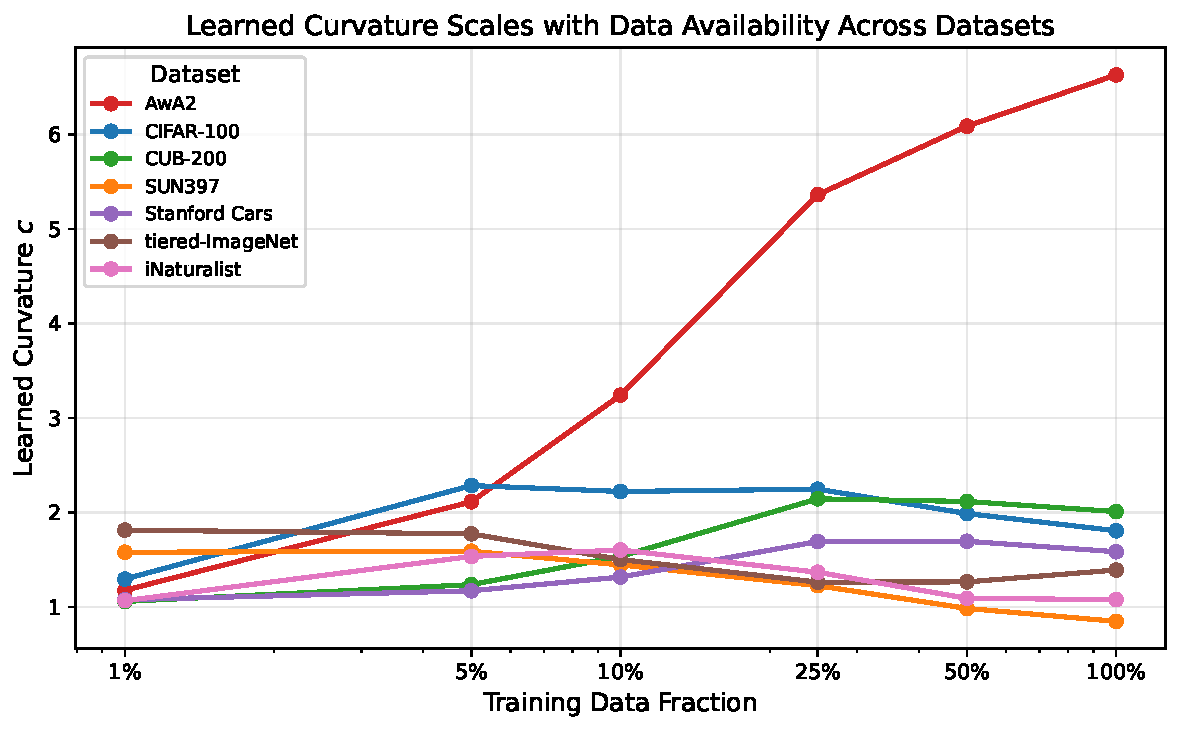
\includegraphics[width=\textwidth]{figures/curvature_vs_data_all.pdf}
\caption{Converged curvature vs.\ training data fraction (log-x) for all seven datasets. AwA2 (top) climbs almost linearly in $\log N$. The GloVe-embedded datasets cluster between $c = 0.8$ and $c = 2.3$ and exhibit qualitatively different trajectories: CUB-200 and Stanford Cars rise then plateau; SUN397, iNaturalist, and tiered-ImageNet peak early and decline.}
\label{fig:curvature_main}
\end{figure}

Fitting a one-line linear model $c = a \log N + b$ separately per dataset gives the slopes in \Cref{tab:logn_fits}.
The signs and magnitudes of $a$ disagree wildly: the AwA2 slope is roughly an order of magnitude larger than CUB-200's (the next-largest positive), and three datasets have \emph{negative} slopes, two of which (SUN397, $a = -0.17$, $R^2 = 0.86$; tiered-ImageNet, $a = -0.13$, $R^2 = 0.75$) fit tightly to clean declines.

\begin{table}[t]
\centering
\caption{Per-dataset fit of $c = a \log N + b$. The slope $a$ varies by an order of magnitude in absolute value and changes sign across datasets, falsifying the universal-scaling claim.}
\label{tab:logn_fits}
\begin{tabular}{lcc}
\toprule
\textbf{Dataset} & \textbf{Slope $a$} & $\boldsymbol{R^2}$ \\
\midrule
AwA2            & $+1.311$ & $0.952$ \\
CUB-200         & $+0.259$ & $0.839$ \\
Stanford Cars   & $+0.145$ & $0.803$ \\
CIFAR-100       & $+0.088$ & $0.151$ \\
iNaturalist     & $-0.028$ & $0.037$ \\
tiered-ImageNet & $-0.126$ & $0.749$ \\
SUN397          & $-0.174$ & $0.858$ \\
\bottomrule
\end{tabular}
\end{table}

\begin{figure}[t]
\centering
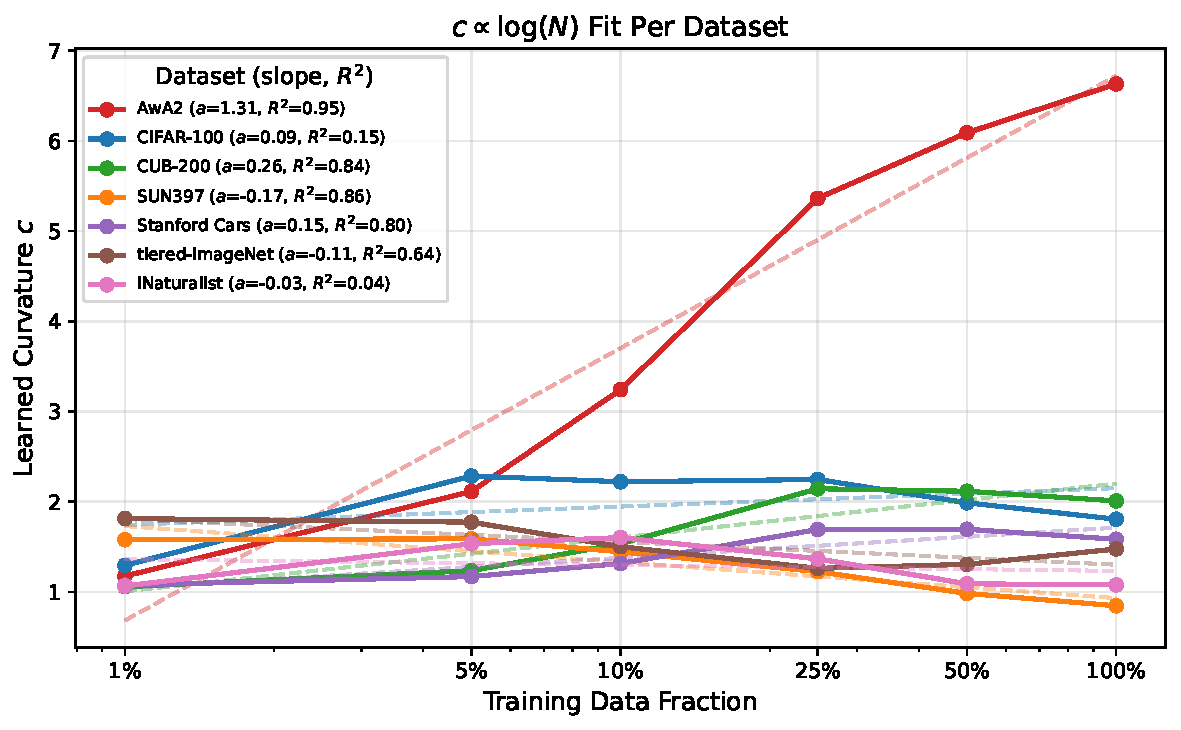
\includegraphics[width=\textwidth]{figures/log_n_fits.pdf}
\caption{Per-dataset $c = a\log N + b$ fits. AwA2's high-$R^2$, high-slope fit is what motivated the original universal-scaling reading. The other six datasets fit either poorly (CIFAR-100, iNaturalist) or to slopes near zero or negative, contradicting that reading.}
\label{fig:log_n_fits}
\end{figure}

\subsection{Three response patterns}\label{sec:patterns}

The within-dataset trajectories in \Cref{fig:curvature_main} cluster into three qualitatively distinct shapes.

\paragraph{Pattern A --- Monotonic increase.}
AwA2 is the sole member: $c$ rises from 1.18 to 6.63, a 5.6$\times$ increase, fitting tightly to a $\log N$ line ($R^2 = 0.95$).
This is the pattern from~\cite{bejleri2025bayesian} that motivated the present study.

\paragraph{Pattern B --- Rises then plateaus.}
CUB-200, Stanford Cars, and CIFAR-100.
All three rise initially (positive slope on the early portion of the sweep), reach a moderate ceiling between $c = 1.7$ and $c = 2.3$ somewhere in the 5--25\% data range, and then stay flat or drift down slightly through 100\% data.
The ceiling is consistent across very different label spaces: CUB-200's deep ornithological hierarchy and Stanford Cars's flat make/model space both produce $c$ around 1.6--2.0 at 100\% data, suggesting the ceiling is not driven by the label hierarchy.

\paragraph{Pattern C --- Peaks then declines.}
SUN397, iNaturalist, and tiered-ImageNet.
Curvature peaks early and \emph{decreases} as more data is added.
SUN397 is the cleanest case: a strict monotonic decline from $c = 1.58$ at 1\% data down to $c = 0.85$ at 100\% --- well below the initial value of $c_0 = 1.0$.
iNaturalist is non-monotonic: a peak of 1.60 at 10\% data followed by a drop back to 1.08 at 100\%.
tiered-ImageNet peaks at the very low end ($c = 1.81$ at 1\% data), declines to a minimum of $c = 1.26$ at 25--50\% data, and shows a small uptick to $c = 1.39$ at 100\% --- still well below the initial peak.

These three patterns describe the data without committing to a mechanism.
The next two subsections explore why they appear.

\subsection{Embedding modality, not taxonomy depth, predicts the pattern}\label{sec:embedding_modality}

\Cref{fig:curvature_vs_hierarchy} shows the converged 100\%-data curvature against the ground-truth tree depth and branching factor of each dataset's taxonomy.
The relationships are weak.
AwA2 (depth 3) and CUB-200 (depth 3) sit at very different curvatures ($c = 6.63$ vs.\ $c = 2.01$).
SUN397 (depth 3), iNaturalist (depth 4), and tiered-ImageNet (depth 5), the three datasets with the deepest taxonomies among the GloVe-embedded ones, are also among the lowest-curvature datasets.
A simple linear regression of $c_{100\%}$ on tree depth across the seven datasets has $R^2 < 0.05$ once AwA2 is excluded, and is essentially driven by AwA2 alone when it is included.

\begin{figure}[t]
\centering
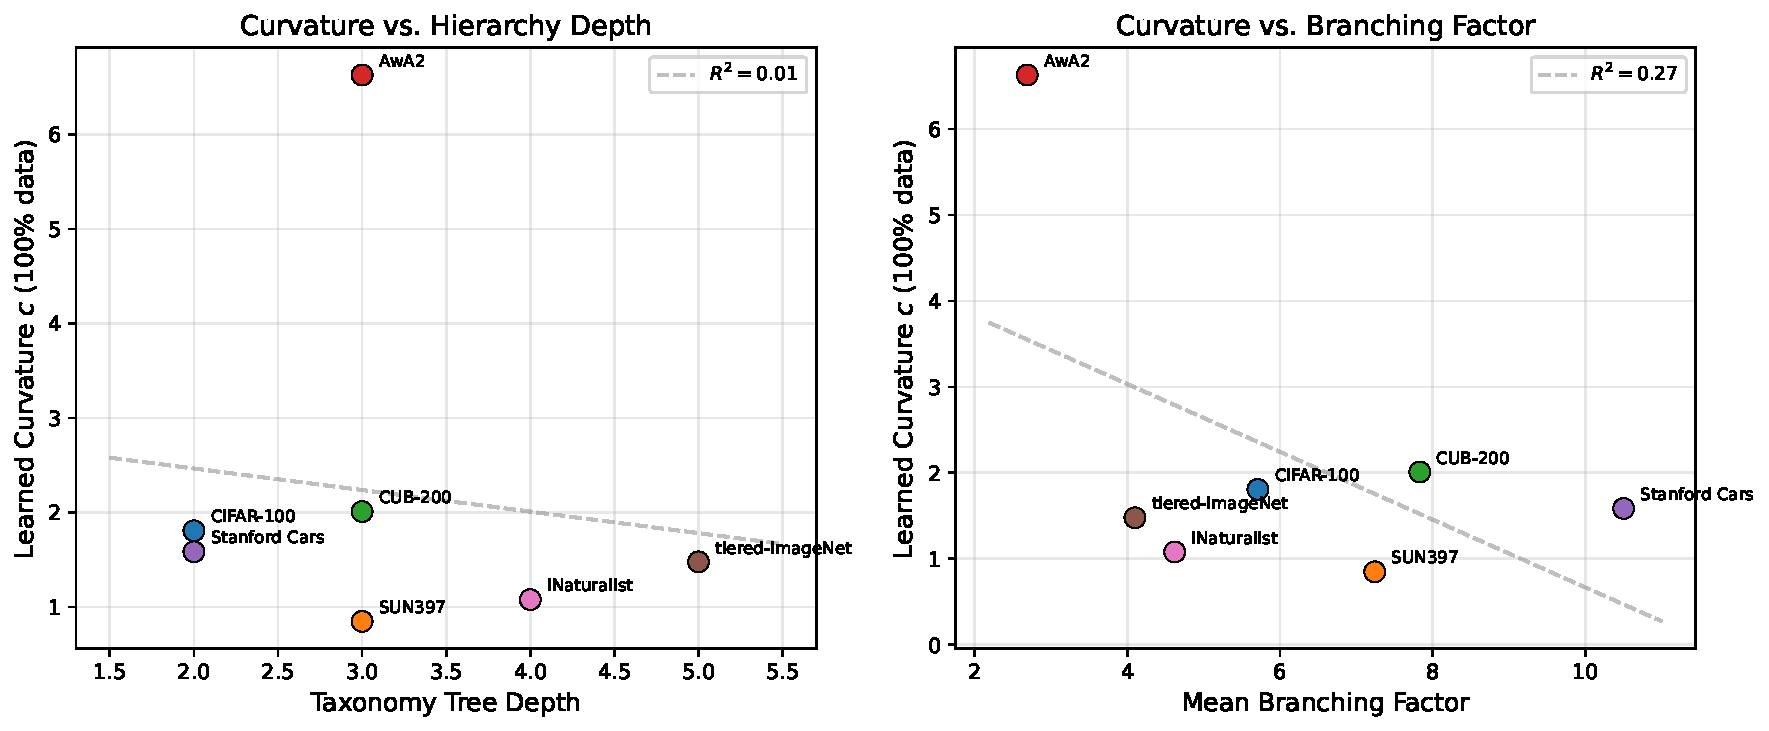
\includegraphics[width=\textwidth]{figures/curvature_vs_hierarchy.pdf}
\caption{Converged curvature at 100\% data vs.\ (left) taxonomy tree depth and (right) mean branching factor. The strong-looking correlations are driven entirely by AwA2 as a single high-curvature outlier; among the six GloVe-embedded datasets, neither metric predicts curvature well.}
\label{fig:curvature_vs_hierarchy}
\end{figure}

The single feature that does predict the pattern cleanly is the embedding modality.
AwA2 (Pattern A, the only outlier) is the only dataset using \textbf{per-class binary attributes}~\cite{xian2018awa2}: 85 expert-annotated dimensions like \texttt{has\_stripes}, \texttt{carnivorous}, \texttt{lives\_in\_water}.
These attributes are chosen by domain experts to maximally discriminate animal species, and they encode rich, structured semantic relationships --- two animals with identical attribute strings would share a complete biological description.
By contrast, the other six datasets use 300-d GloVe word vectors derived from class names (or, for tiered-ImageNet and iNaturalist, from taxonomy-derived words).
GloVe vectors are trained on co-occurrence statistics in unstructured text and capture mostly distributional similarity; they do not encode the kind of fine-grained discriminative structure that per-class attributes do.

This distinction predicts:
\begin{itemize}
    \item Pattern A appears only when the class embeddings are themselves richly structured. AwA2's curvature climbs because each new training example refines the alignment of visual features with a meaningful, dense per-class semantic description, and the model can keep extracting more geometric structure from the data.
    \item Patterns B and C appear when the class embeddings are flatter (in the structural sense) than the visual features. The model learns a useful curvature in the small-data regime --- when class embedding distances are the only available signal --- but as visual features become individually informative (with more data), it discovers that compressing into curved space buys it less than letting the visual encoder do the discrimination directly. This produces the plateau (Pattern B) or, on visually rich datasets with many classes (SUN397, iNaturalist), the active decline (Pattern C).
\end{itemize}
We do not claim this explanation is the only one consistent with the data.
But the magnitude of the AwA2 vs.\ everything-else gap (a factor of roughly 4$\times$) cannot be explained by taxonomy alone, given that CUB-200's depth-3 ornithological hierarchy and CIFAR-100's depth-2 superclass structure both produce curvatures in the same modest range as Stanford Cars's flat make space.

\subsection{Number of classes interacts with the pattern}\label{sec:n_classes_effect}

A secondary observation: the three datasets in Pattern C (declining curvature) are also our three largest by class count: SUN397 (397), iNaturalist (500), and tiered-ImageNet (608).
CUB-200 (200) sits at the boundary --- its 100\%-data curvature ($c=2.01$) is below its 25\%-data peak ($c=2.14$), but only marginally.
A plausible reading is that with hundreds of classes embedded into 300-d GloVe space, many class embeddings end up near each other (especially fine-grained taxonomic classes whose names share roots), and large-curvature embeddings then exaggerate noise rather than signal.
The model unlearns its initial curvature to compensate.
This explanation is consistent with tiered-ImageNet (608 classes drawn from WordNet leaves whose lemmas often duplicate or differ by a single qualifier) showing the lowest peak curvature among the GloVe-embedded large datasets and the steepest early decline.

\subsection{Comparison with Fan et al.}\label{sec:fan_comparison}

Fan et al.~\cite{fan2025curvature} report converged curvature values from a sharpness-aware bi-level optimisation procedure on a few-shot classification objective.
Their reported $c \approx 0.113$ on tiered-ImageNet 1-shot is roughly an order of magnitude smaller than our converged values on the same dataset (which range from $c = 1.26$ at 25--50\% data to $c = 1.81$ at 1\% data, ending at $c = 1.39$ at 100\%).
Our setup uses a different training objective (ZSL geodesic alignment), a different evaluation protocol, and a different curvature parameterisation, so a precise numerical comparison is not meaningful.
What is meaningful is that both papers find tiered-ImageNet's optimal/converged curvature in a low-to-moderate range that does not grow without bound with more data --- consistent with the more general observation that text-derived class embeddings on large class sets produce only moderate curvature, in striking contrast to AwA2's attribute-driven climb to $c = 6.63$.

A more important point: our results suggest that ``optimal curvature for tiered-ImageNet'' is best understood as ``optimal curvature for tiered-ImageNet \emph{when classes are encoded by GloVe word vectors}.''
A different class encoding --- per-class attributes, learned visual prototypes, language-model embeddings --- would likely produce a different optimum.
Prescriptive curvature-tuning procedures should report (and ideally vary) the embedding modality alongside the dataset.

% ================================================================
%  6. DISCUSSION
% ================================================================
\section{Discussion}\label{sec:discussion}

\paragraph{Curvature reports semantic structure as the model can see it.}
The picture that emerges is not ``curvature reports the dataset's hierarchy depth.''
It is ``curvature reports how much hierarchical/relational structure the model can extract from its inputs given how the classes are encoded.''
On AwA2, that structure is rich and the model keeps finding more of it as data grows.
On GloVe-embedded datasets, the structure available through 300-d word vectors is shallower, and the model converges to a moderate curvature ceiling --- or, when the class set is large enough that GloVe distances stop being discriminative, retreats from curvature entirely.

\paragraph{Implications for hyperbolic network design.}
A practical consequence: when designing a hyperbolic network for a new task, the choice of class embedding may matter as much as the choice to use hyperbolic geometry.
A hyperbolic network with weak class embeddings may end up learning a near-Euclidean curvature in any case, defeating the purpose of the architectural choice.
Practitioners might reasonably treat the converged curvature as a diagnostic: if $c$ stays near $c_0$ or drops below it, the embedding likely lacks the structure the geometry was meant to exploit, and either the embedding or the architecture should be reconsidered.

\paragraph{Why does AwA2 keep climbing?}
The $c$ values for AwA2 do not plateau within our 100\% data sweep, raising the question of whether they would saturate at higher data --- noting that AwA2 has only $\sim$30K images, so we cannot push much further on this dataset alone.
Our reading is that the saturation point of Pattern A is determined by the resolution of the per-class semantic description, not by the visual signal: AwA2's 85-d attribute vectors carry roughly $\log_2(85!) \approx 350$ bits of class-discriminative information assuming uncorrelated dimensions, and the model's curvature continues climbing as long as additional data lets it discover finer divisions of that structure.
Datasets with even richer per-class descriptions (e.g., long natural-language captions, multi-modal embeddings) might produce even steeper Pattern A curves.

\paragraph{What about $\delta$-hyperbolicity?}
We computed taxonomy-derived hierarchy metrics (depth, branching factor) but did not include feature-space $\delta$-hyperbolicity~\cite{gromov1987hyperbolic,fournier2015hyperbolicity} in the main analysis.
A natural extension is to compute $\delta$ on the joint visual-feature plus class-embedding metric and see whether it correlates with the converged curvature better than taxonomy depth does --- particularly since $\delta$-hyperbolicity is sensitive to the embedding metric in a way that taxonomy depth is not.

\paragraph{Limitations.}
Seven datasets is a thin slice of the space.
The strong reading of our embedding-modality claim --- that attribute embeddings always produce Pattern A and word-vector embeddings never do --- is single-anchor in our data: AwA2 is the only dataset with attributes, so we cannot distinguish ``attributes cause Pattern A'' from ``some other AwA2-specific factor causes Pattern A.''
A direct test would re-run the same architecture on AwA2 with GloVe embeddings of the class names (e.g., \texttt{tiger}, \texttt{antelope}) instead of the attribute matrix, and see whether the curvature trajectory drops to a Pattern B or Pattern C shape.
We mark this as future work.

% ================================================================
%  7. CONCLUSION
% ================================================================
\section{Conclusion}\label{sec:conclusion}

We tested whether the $c \propto \log N$ scaling of learned Poincar\'{e} ball curvature observed on AwA2 generalises across image classification datasets.
It does not.
Across seven datasets, the within-dataset slope of $c$ vs.\ $\log N$ varies from $+1.31$ (AwA2) to $-0.17$ (SUN397), and the trajectories cluster into three distinct response patterns.
The strongest predictor of which pattern a dataset exhibits is the type of class embedding used --- per-class attributes (AwA2) versus word vectors (everything else) --- and not the depth of the underlying taxonomy.
We re-frame the descriptive question accordingly: learned curvature reports the dataset's semantic structure \emph{as visible through its embedding modality}, not its taxonomy.

% ================================================================
%  REFERENCES
% ================================================================
\bibliographystyle{plainnat}
\bibliography{references}

\end{document}
